
%%% Local Variables:
%%% mode: latex
%%% TeX-master: t
%%% End:

\chapter{引言}
\label{chap:intro}

互联网与云计算的发展,越来越多的应用从本地迁移到云端,并涌现出大量新兴的互联网应用,
承载这些应用的数据中心成为了如同电力系统一样的社会基础设施。
与此同时,现代数据中心正在面临着权衡资源利用率与应用服务质量的挑战:
从应用开发者角度,服务质量是第一位的,因为它直接关系到用户体验与其收益,
由于互联网应用负载的波动性,开发人员通常会为自己的应用过量分配资源以满足峰值时的负载需求,
这造成了非常低的服务器利用率,通常只有6\%-12\%;
而对于数据中心运维人员,资源利用率直接反映其运维成本,虽然将不同应用混合部署到同一台服务器,
充分利用空闲时段的服务器资源可以有效提高数据中心利用率,
但多应用混合部署引入的软硬件资源共享会造成应用间无管理的资源竞争,
使得应用性能出现不可预测的波动,进而影响应用的服务质量。
由上可知,如何权衡数据中心资源利用率与应用服务质量是当前数据中心亟待解决的重要问题。

可以从三个角度解决这一问题:
其一是通过上层软件机制实现干扰容忍,在应用层保障服务质量,
如Google提出的Hedged Requests和Tied Requests方案\cite{dean_tail_2013},
通过向多个副本发送请求,并选择最快返回的结果以达到干扰容忍的目的。%Timecard和D2P
其二是在应用调度层次,通过profile的方式预测应用混合后的干扰情况,
将相互之间干扰较小的应用部署到同一台服务器。
其三是提供一个良好的隔离环境,降低由资源竞争所产生的应用间干扰,
可以在各个层次实现隔离,如操作系统级\cite{cgroup}、Hypervisor级\cite{}、硬件级\cite{}。

其中前两种方案在实施时需要对目标应用具有非常深入的理解:
方案一需要对应用架构与实现细节进行修改,以达到应用层干扰容忍的目的;
方案二虽然无需对应用进行修改,但需要对应用的资源占用以及不同应用之间的干扰状况进行分析,
才能得到最优的调度方案。
当应用数量不多且有条件进行以上所述的分析或修改,通过精细的应用架构设计与调度机制,
可以有效的解决前文所提到的资源利用率与服务质量相冲突的问题。
但在现实数据中心特别是云计算数据中心内,以上假设并不成立。

首先,数据中心内通常会运行大量的应用,如Google的数据\cite{}表明其数据中心在两个月内累计运行超过2000000个应用,
无论是改造这些应用或是对应用之间的干扰行为进行分析都是不可行的。
即使只对部分关键的应用进行改造使其适应干扰环境,云计算环境下的“吵闹的邻居(Noisy Neighbors)”也会使这些努力的结效果大打折扣。

其次,调度方案无法解决短时运行的干扰应用对其它正常应用带来的影响,特别是随着DevOps的兴起,
由于开发调试与线上部署是不断迭代进行的,调试过程中所引入的短时干扰应用数量大大增加,
Google的数据\cite{}发现大量的小于6分钟的应用都是来自于这些调试应用。
当调度器发现干扰并准备采取调度措施时干扰应用可能已经结束,同时新的干扰应用又开始运行,并带来新的干扰。

当前对第三种隔离方案也有很多研究,包括在软件栈各个层次如虚拟化层\cite{}、操作系统内核层\cite{}、网络协议栈\cite{}等的隔离。
由于在软件层次只能做到较粗粒度的资源管理,实现的效果有限;
同时应用的不同特征造成资源竞争点是分布在整个软件栈中,因此只能根据实际场景做针对性的优化;
再次,在如此复杂的软件栈中找到真正的资源竞争点需要大量的时间与精力,这同样不能满足云计算的场景下应用多样与快速部署的需求。
除了软件栈上的共享,混合部署的应用在硬件层次上也存在大量的共享,如CPU末级缓存、内存控制器、I/O等,
另一些研究专注于如何在这些共享硬件上提供隔离功能,典型的工作如末级缓存划分\cite{}和内存控制器划分\cite{},
但这些研究大都只关注于一种类型的资源,而且是针对特定的场景,因此缺少灵活的软件编程接口,不能适用于通用的计算场景。

综上可知,现有的三种方案都不能很好的解决当前云计算数据中心中遇到的资源利用率与服务质量矛盾的问题,
这一问题的本质是如何为应用提供区分化服务,而如何解决目前计算机系统的软硬件资源的无管理共享状态是实现区分化服务的关键。
现有研究在一定程度上能够解决软件层次的共享管理问题,但无管理的硬件共享使得这一问题并没有被完全解决。
造成这一现状的原因是目前的计算机体系结构在设计时并没有考虑到多应用共享场景,
其使用的指令集抽象不足以将上层应用需求传递到下层硬件,在不能区分应用需求的前提下很难做到区分化服务。
软件层次已有很多方案可以用于区分不同应用,如操作系统级的进程PID或cgroup,或更细粒度的应用级标签。%\cite{zhangxd:software-defined-storage, timecard, d2p, ...}
硬件层次也需要一种应用需求传递机制,正如“21st Century Computer Architecture”白皮书中所提出的:

\begin{quotation} 
\emph{\textbf{Better Interfaces for High-Level Information.}
Current ISAs fail to provide an efficient means of capturing software-intent or conveying critical high-level information to the hardware.
For example, they have no way of specifying when a program requires energy efficiency, robust security, or a desired Quality of Service (QoS) level.
Instead, current hardware must try to glean some of this information on its own ......
% - such as instruction-level parallelism or repeated branch outcome sequences - at great energy expense. 
\textbf{New, higher-level interfaces are needed to encapsulate and convey programmer and compiler knowledge to the hardware,}
resulting in major efficiency gains and valuable new functionality.}\cite{21st_architecture}
\end{quotation}

因此要实现高效通用数据中心目标,核心是从硬件上改变资源的“无管理共享”现状以实现在体结构上支持应用服务质量保障,在
此基础上实现数据中心资源根据应用动态管理以提高资源利用率。

\begin{figure}[H]
  \centering
  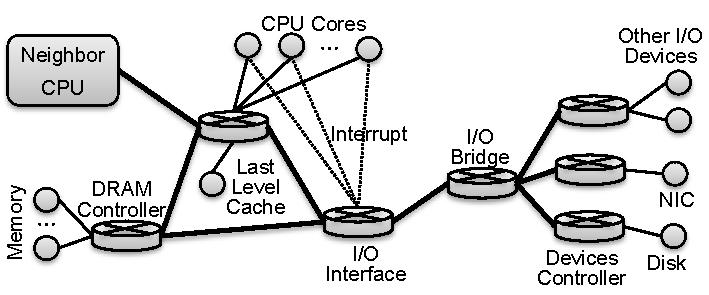
\includegraphics[height=4cm]{intro/computer-as-a-network.pdf}
  \caption{计算机内部网络}
  \label{fig:computer-as-a-network}
\end{figure}

本文提出了PARD\cite{pard2015}技术,扩展现有体系结构实现应用需求在整个计算机系统传播,并通过细粒度的硬件资源管理,
实现体系结构支持的服务质量保障。PARD体系结构的核心是基于一个重要的观察:计算机内部是一个网络。
如图\ref{fig:computer-as-a-network}所示,CPU核、共享缓存、内存控制器、I/O设备等可以被看做是网络节点;
除了处理请求以外,这些“网络节点”与网络中的路由器/交换机具有相似的请求转发功能;
而它们之间也通过包进行通信,如:片内通信使用NoC包,片间通信的QPI/HT包,以及I/O部分使用的PCI-E包。

而在网络上如何实现端到端的服务质量保障已有大量的研究,并已形成标准,
如IETF(Internet Engineering Task Force, 互联网工程任务组)于1998年提出了区分化服务(Differentiated Services)的概念,
如今区分化服务已经成为应用最广泛的服务质量保障机制之一。
该技术的核心是在IP包头中定义长度为8-bit的区分化服务域,用以表示应用的
服务质量分类标识,因此路由器、交换机等网络设备便可以使用该信息对不同类别的数据包
进行区分处理,以达到区分化服务的目的。
软件定义网络(SDN)的出现,进一步促进了网络领域服务质量保障的发展,
其主要原理可以概括为:(1) 控制平面与数据平面分离;(2)集中控制的统一编程接口。
将网络领域的区分化服务和软件定义网络的思想应用到计算机内部的网络,
用以解决数据中心当前面临的资源利用率与应用服务质量矛盾,是本文的主要研究思路与动机。

\section{论文的主要贡献}
In this paper, we propose Programmable Architecture for
Resourcing-on-Demand (PARD) that provides a new programming
interface to convey an application’s QoS requirements to the hardware.
PARD supports new functionalities such as fully hardwaresupported
virtualization without software hypervisors and differentiated
service (DiffServ) [60] in data center servers. For instance,
PARD can accurately isolate performance in shared data centers
to improve server utilization without degrading QoS for latencycritical
applications.


\section{论文的组织结构}

本文共分八章,第一章介绍移动计算带来的新计算模式对数据中心的挑战,然后讨论现有
数据中心技术的局限性,并针对现有体系结构提出了新的需求,最后介绍了论文的研究动机、
主要贡献和组织结构。

第二章介绍体系结构领域解决服务质量问题的现有研究,并对比以网络领域的相关内容,
讨论两者相互借鉴的可能性。

第三章对现有体系结构的服务质量支持进行评估,包括软件(cgroup, hyperviso)和硬件
两个层次。

第四章介绍资源管理可编程体系结构的概念与核心思路,并将其映射到现有体系结构,
讨论其可行性。同时应用资源管理可编程体系结构实现全硬件虚拟化,并讨论其关键技术。

第五章讨论模拟器实现,主要从功能设计角度对控制面设计,与资源管理可编程实现,
硬件支持、Trigger-Action机制,模拟的方式验证PARD的有效性。

第六章基于前两章的设计给出本文资源管理可编程体系结构的FPGA原型系统实现,
并对原型系统各部分功能的正确性、性能与开销进行了详细评测。

第七章在数据中心场景下,对本文资源管理可编程体系结构在分布式场景下应用进行讨论。

第八章总结全文并介绍未来可能的研究工作。
